% vim: ft=tex
\chapter{Scope}
TODO what's this thesis about

\section{Motivation}
TODO Why do we care about this thesis? Why are we interested?

\section{Initial Situation}
TODO What's Roadster and its goals

\subsection{Software Architecture}
TODO Roadster architecture\\

\subsubsection{ZeroMQ}
To be able to understand Roadster's architecture, it's helpful to understand
the basics of ZeroMQ (hereafter ZMQ) first. This is a brief introduction to ZMQ
for the unfamiliar reader.\\

ZMQ is a message oriented middleware implemented as a library (it doesn't
require a broker). Instead, it provides a set of unique socket types and a very
abstract, simple interface to interact with them. Socket types:\\

\begin{description}
	\item [REQ and REP] strict request-reply message handling (synchronous
		and thus fragile and unflexible)

	\item [DEALER and ROUTER] similar, but doesn't enforce strict
		request-reply fashion (asynchronous and thus more robust and
		flexible)

	\item [PUB and SUB] publish-subscribe

	\item [PUSH and PULL] fan in/fan out, useful for pipelines, round
		robbin on sender side, fair queueing on receiver side
\end{description}

TODO not strictly server/client type: order of bind/connect doesn't matter\\
TODO binding/connecting a socket to multiple endpoints is possible\\
TODO a single socket for many connections, connection handling is completely abstracted away\\
TODO supported transports: in-memory, IPC, TCP, multicast (UDP or TCP?), TIPC\\
TODO to achieve reliability or any custom message flow desirable, you build your own solution using this library, see zguide.\\
(TODO security)\\
(TODO CZMQ abstraction layer)\\

It is several orders of magnigude more performant than other well known MOMs,
including closed source and open source solutions.\\

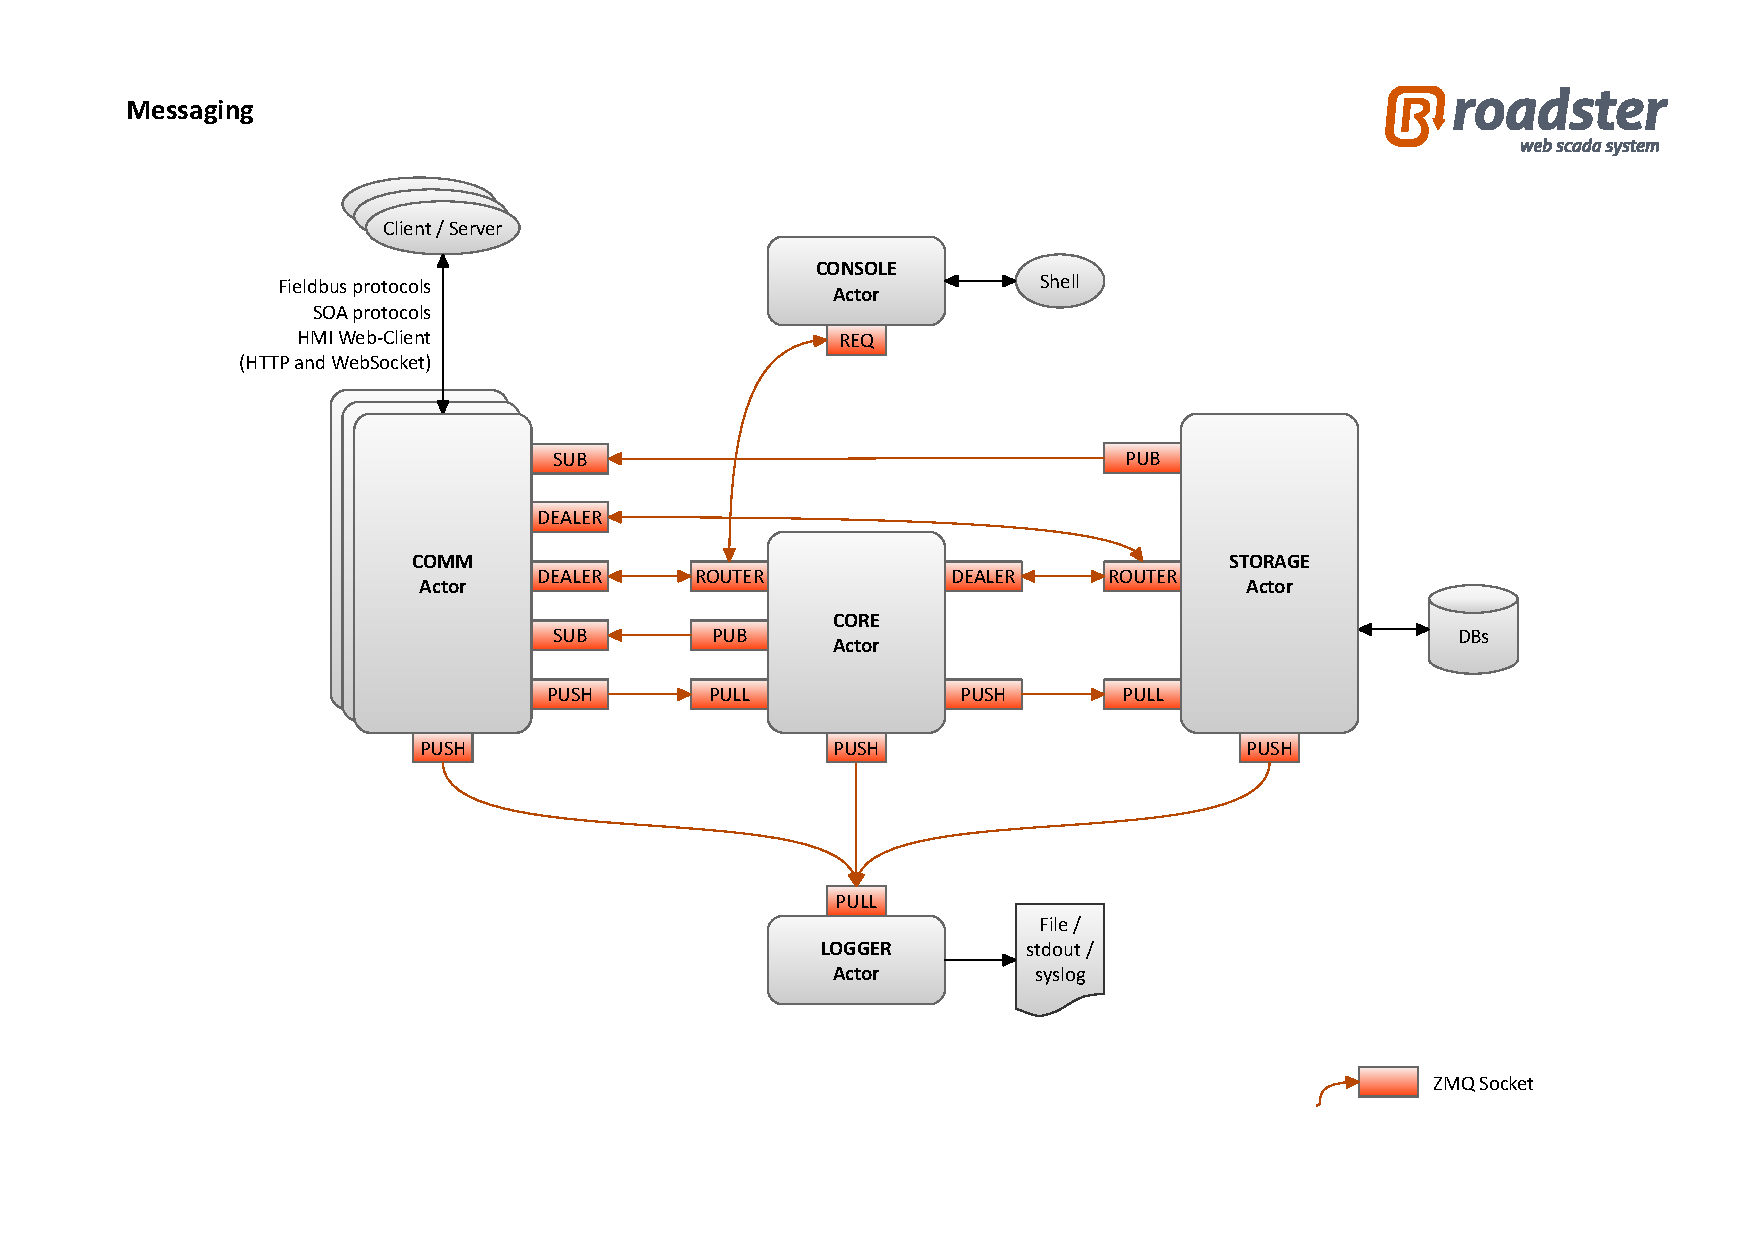
\includegraphics[trim=4cm 2cm 3.5cm 2.8cm, clip=true, width=\textwidth]{img/roadster_arch.pdf}

\section{Goals}
TODO mandatory goals

\subsection*{Optional Goals}
TODO optional goals
